\begin{figure}[ht]
\centering
\begin{subfigure}[t]{0.4\linewidth}
  \centering
  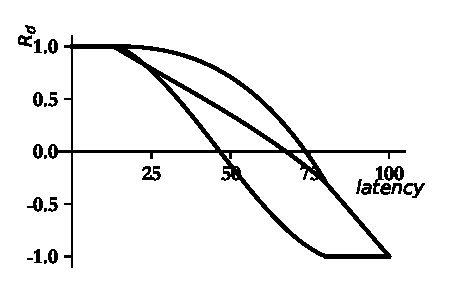
\includegraphics[width=\linewidth]{figures/chap03/reward_function/Rd.pdf}
  \caption{延迟奖励}
  \label{fig:Latency Reward}
\end{subfigure}%
\hspace{0.05\linewidth} % 添加水平间距
\begin{subfigure}[t]{0.4\linewidth}
  \centering
  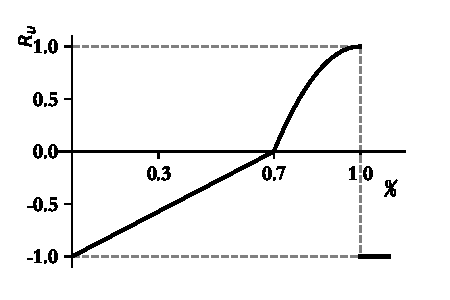
\includegraphics[width=\linewidth]{figures/chap03/reward_function/Ru.pdf}
  \caption{带宽利用率奖励}
  \label{fig:Bandwidth Utilization Reward}
\end{subfigure}

\vspace{0.5em} % 适当增加垂直间距
\begin{subfigure}[t]{0.4\linewidth}
  \centering
  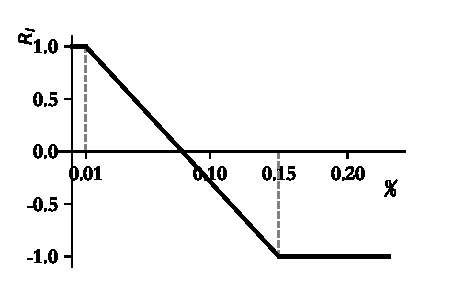
\includegraphics[width=\linewidth]{figures/chap03/reward_function/Rl.pdf}
  \caption{丢包率奖励}
  \label{fig:Loss Ratio Reward}
\end{subfigure}%
\hspace{0.05\linewidth} % 添加水平间距
\begin{subfigure}[t]{0.4\linewidth}
  \centering
  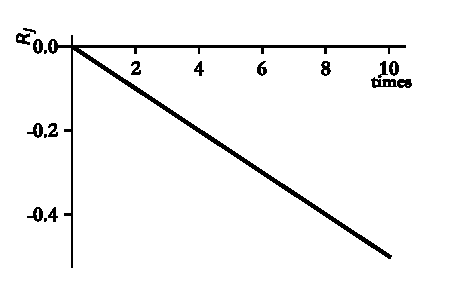
\includegraphics[width=\linewidth]{figures/chap03/reward_function/Rj.pdf}
  \caption{屏幕抖动奖励}
  \label{fig:jitter Reward}
\end{subfigure}

\caption{强化学习中的奖励函数构成}
\label{fig:reward-function}
\end{figure}
